% generated by roam.py handbook export -- не редактировать, править заметки
% 20261010100732-метопт_лекция_3_начало_оптимизации.org

\chapter{Начало оптимизаций}\label{lecture:3}
\InputIfFileExists{text/03-intro}{}{}

\section{Введение: термины}\label{lecture:3:1}  % конспект 3.1
\InputIfFileExists{text/03-1-intro}{}{}

\noteagain{655064DF-D686-4726-83DC-6F3D67CC5B9C}{Оценка для выпуклых функций с липшицевым градиентом}  % -- замечание 3.1 («было»), в частности $\frac{1}{2L}\|\nabla f(y)\|^2 \le f(y) - f(x^{*})$

\InputIfFileExists{text/C42D2C19-B35F-4C0E-AFEB-D880CBB72176-before}{}{}
% generated by roam.py handbook export -- не редактировать, править заметки
% 20261004142030-невязка.org (body baf08f632457)

\begin{definition}[{Невязка}]\label[definition]{note:C42D2C19-B35F-4C0E-AFEB-D880CBB72176}
  Невязка~--- величина, отвечающая за измерение близости к точке оптимума.
  Обозначается как $r_k$.

  Виды невязок (где $x^{*}$~--- точка оптимума):

  \begin{itemize}
    \item $r_k = \| x^{*} - x_{k}\|_2$
    \item $r_k = |f(x_k) - f(x^{*})|$
    \item $r_k = \| \nabla f(x_k)\|_2$
  \end{itemize}

  Шаг постоянный ($\alpha_k = 1/L$), по конспекту:

  \begin{center}
  \begin{tabular}{l l l}
    \hline
    Класс функций & Невязка & Сходимость \\
    \hline
    $f \in C^{1,1}_L$ & $\norm{\nabla f(x_k)}$ & $c/\sqrt{k}$ (\hyperref[note:C3B64D64-D35B-42AC-B683-6736227CBBBC]{теорема}) \\
    $f \in C^{1,1}_L$, $\mu$-сильно выпуклая & $\norm{x_k - x^{*}}^2$ & $(1 - \mu/L)^k$ (\hyperref[note:85D9D77D-13A2-42E0-BF93-AD085E0134B9]{теорема}) \\
    $f \in C^{1,1}_L$, выпуклая & $f(x_k) - f^{*}$ & $c/k$ (без доказательства) \\
    \hline
  \end{tabular}
  \end{center}
\end{definition}
  % Невязка -- обозначение $r_k$ перед опр. 3.1; таблица «Шаг постоянный» (стр. 9)

\InputIfFileExists{text/55E52506-D4CB-4D20-AB2E-3793825A406F-before}{}{}
% generated by roam.py handbook export -- не редактировать, править заметки
% 20261004142559-скорость_сходимости.org (body 7c0a208a6f37)

\begin{definition}[{Скорость сходимости}]\label[definition]{note:55E52506-D4CB-4D20-AB2E-3793825A406F}
  Скорость сходимости итерационного метода~--- то, как быстро убывает \hyperref[note:C42D2C19-B35F-4C0E-AFEB-D880CBB72176]{невязка} $r_k \to 0$ (здесь $r_k > 0$). Виды:

  \begin{enumerate}
    \item \hyperref[note:DF2405BF-8B31-47EB-8DEF-B1A88034717C]{Линейная сходимость}
    \item \hyperref[note:A74C35E2-DDF7-4115-99B7-2448CF7C6878]{Сублинейная сходимость}
    \item \hyperref[note:9FA20DA5-3A95-4683-9CB5-C6C9A903C86A]{Сверхлинейная сходимость}
  \end{enumerate}
\end{definition}
  % Скорость сходимости -- опр. 3.1

\InputIfFileExists{text/DF2405BF-8B31-47EB-8DEF-B1A88034717C-before}{}{}
% generated by roam.py handbook export -- не редактировать, править заметки
% 20261004142614-линеиная_сходимость.org (body 5cbe2a2e4acf)

\begin{definition}[{Линейная сходимость}]\label[definition]{note:DF2405BF-8B31-47EB-8DEF-B1A88034717C}
  Последовательность $r_k$~--- \hyperref[note:C42D2C19-B35F-4C0E-AFEB-D880CBB72176]{невязок}~--- сходится \emph{линейно}, если $\exists C > 0,\ q \in (0;1)$ такие, что
  $r_k \le Cq^k$ для любого $k \in \N_{0}$
\end{definition}

\begin{remark}
  $\log_{10} r_k \le \log_{10} C + k \log_{10} q$~--- число верных десятичных знаков растёт линейно по $k$; отсюда название.
\end{remark}
  % Линейная сходимость -- опр. 3.1 (1), замечание 3.2 — в /Rem/

\InputIfFileExists{text/A74C35E2-DDF7-4115-99B7-2448CF7C6878-before}{}{}
% generated by roam.py handbook export -- не редактировать, править заметки
% 20261004142830-сублинеиная_сходимость.org (body 6453a1da8c74)

\begin{definition}[{Сублинейная сходимость}]\label[definition]{note:A74C35E2-DDF7-4115-99B7-2448CF7C6878}
  Последовательность $r_k \to 0$~--- \hyperref[note:C42D2C19-B35F-4C0E-AFEB-D880CBB72176]{невязок}~--- сходится \emph{сублинейно}, если она не сходится \hyperref[note:DF2405BF-8B31-47EB-8DEF-B1A88034717C]{линейно}. Пример: $r_k = \frac{1}{k}$.
\end{definition}
  % Сублинейная сходимость -- опр. 3.1 (2)

\InputIfFileExists{text/9FA20DA5-3A95-4683-9CB5-C6C9A903C86A-before}{}{}
% generated by roam.py handbook export -- не редактировать, править заметки
% 20261004142956-сверхлинеиная_сходимость.org (body 48db6bc08313)

\begin{definition}[{Сверхлинейная сходимость}]\label[definition]{note:9FA20DA5-3A95-4683-9CB5-C6C9A903C86A}
  Последовательность $r_k$~--- \hyperref[note:C42D2C19-B35F-4C0E-AFEB-D880CBB72176]{невязок} сходится \emph{сверхлинейно}, если она сходится \hyperref[note:DF2405BF-8B31-47EB-8DEF-B1A88034717C]{линейно}
  для любого $q \in (0;1)$

  Пример: $r_k = q^{k^2}$ или $r_k = 1/k!$. Достаточно, чтобы $r_{k+1}/r_k \to 0$.
\end{definition}
  % Сверхлинейная сходимость -- опр. 3.1 (3)

\InputIfFileExists{text/C0408924-F658-43DF-8794-0C9AA85E7580-before}{}{}
% generated by roam.py handbook export -- не редактировать, править заметки
% 20261004145821-тест_корнеи.org (body cdb88c7620cf)

\begin{theorem}[{Тест корней}]\label[theorem]{note:C0408924-F658-43DF-8794-0C9AA85E7580}
  Пусть $r_k > 0$, $r_k \rightarrow 0$, $a := \limsup_{n\rightarrow\infty} \sqrt[n]{r_n}$

  Если:

  \begin{enumerate}
    \item $0 \le a <1$, то $r_k$~--- сходится \hyperref[note:DF2405BF-8B31-47EB-8DEF-B1A88034717C]{линейно}
    \item $a = 0$, то $r_k$~--- сходится \hyperref[note:9FA20DA5-3A95-4683-9CB5-C6C9A903C86A]{сверхлинейно}
    \item $a = 1$, то $r_k$~--- сходится \hyperref[note:A74C35E2-DDF7-4115-99B7-2448CF7C6878]{сублинейно}
  \end{enumerate}
\end{theorem}

\begin{remark}
  Можно использовать и $\lim \frac{r_{k+1}}{r_k}$ (если этот предел существует, он равен $a$) по Даламберу
\end{remark}

\begin{remark}
  Условие $r_k \to 0$ гарантирует $a \le 1$ (с некоторого момента $r_k < 1$), так что три случая исчерпывают всё.
\end{remark}

\begin{proof}
  \proofpart{1}
  Возьмем произвольное $q$, такое, что $a < q < 1$.
  Тогда, начиная с некоторого момента $N$, $\forall k \ge N\ \sqrt[k]{r_k} < q$, то есть $r_k < q^k$

  Для остальных $n < N$ заведем константу $C$ такую, что
  \[
  C = \max \left( 1, \max_{n < N} \frac{r_n}{q^n} \right)
  \]
  Тогда $\forall n\  r_n \le Cq^n$

  \proofpart{2}
  Если взять $a = 0$, то доказательство 1 будет верно для $\forall q \in (0;1)$, что и соответствует
  определению \hyperref[note:9FA20DA5-3A95-4683-9CB5-C6C9A903C86A]{сверхлинейной сходимости}.

  \proofpart{3}
  Пойдем от обратного; Пусть $a = 1$ и $\exists C, q:\  \forall n\ r_n \le Cq^n$ \\
  При этом $q \in (0;1), C>0$.

  У нас есть оценка
  \[
  r_n \le C q^n \Rightarrow \sqrt[n]{r_n} \le C^{\frac{1}{n}} q \rightarrow q < 1
  \]
  Но при этом $\limsup \sqrt[n]{r_n} = a = 1$.
  Противоречие
\end{proof}
  % Тест корней -- нет в конспекте

\InputIfFileExists{text/BEEE81AD-13FC-4846-A160-C72E31760BEE-before}{}{}
% generated by roam.py handbook export -- не редактировать, править заметки
% 20261004152534-виды_градиентного_спуска.org (body 42d7cb5f0033)

\begin{concept}[{Виды градиентного спуска}]\label[concept]{note:BEEE81AD-13FC-4846-A160-C72E31760BEE}
  Рассмотрим общую схему метода спуска из точки $x_k$:
  \[
  x_{k+1} = x_k + \alpha_kd_k
  \]
  Где: $d_k$~--- направление спуска,  $\alpha_k$~--- шаг спуска.

  Как выбрать шаг спуска:

  \begin{enumerate}
    \item Фиксированный шаг
    \item \hyperref[note:8EDDABAC-D2BE-4EC9-8297-DBAC52F70D28]{Точная одномерная оптимизация} $\alpha_k = \arg\min_{\alpha > 0} f(x_k + \alpha d_k)$
    \item \hyperref[note:A818191F-B1A6-492C-B38D-5369D169161C]{Неточная одномерная оптимизация}: не обязательно на каждом шаге искать идеальное решение. Пример: \hyperref[note:5330B23D-95DD-4D5D-B4A3-63EBADB1DB7D]{условия Армихо-Вульфа}.
  \end{enumerate}
\end{concept}

\begin{remark}
  При $d_k = -\nabla f(x_k)$ это градиентный спуск.
\end{remark}
  % Виды градиентного спуска -- рассуждение 3.1

\InputIfFileExists{text/950F2C19-C2C7-42CD-9CDF-0B9AC03A3DC8-before}{}{}
% generated by roam.py handbook export -- не редактировать, править заметки
% 20261010095611-порядок_метода_оптимизации.org (body 0c279e92f336)

\begin{definition}[{Порядок метода оптимизации}]\label[definition]{note:950F2C19-C2C7-42CD-9CDF-0B9AC03A3DC8}
  Метод оптимизации называют методом \emph{$k$-го порядка}, если он использует производные $f$ до $k$-го порядка включительно:

  \begin{itemize}
    \item метод \emph{нулевого порядка}~--- только значения функции (например, \hyperref[note:96DED7D9-3918-45C5-9850-E05030941645]{метод золотого сечения}, \hyperref[note:4E950058-62DB-4EDA-A71D-98CACBBC41AA]{метод парабол});
    \item метод \emph{первого порядка}~--- значения и градиент (например, \hyperref[note:124BD9BC-084E-43FB-B617-AF8690B33EF8]{дихотомия по производной}, \hyperref[note:BEEE81AD-13FC-4846-A160-C72E31760BEE]{градиентный спуск});
    \item метод \emph{$k$-го порядка}~--- $f^{(k)}$.
  \end{itemize}
\end{definition}
  % Порядок метода оптимизации -- опр. 3.2

\section{Одномерная оптимизация: точные методы}\label{lecture:3:2}  % конспект 3.2.1
\InputIfFileExists{text/03-2-intro}{}{}

\InputIfFileExists{text/8EDDABAC-D2BE-4EC9-8297-DBAC52F70D28-before}{}{}
% generated by roam.py handbook export -- не редактировать, править заметки
% 20261004180905-точная_одномерная_оптимизация.org (body 296c8df052df)

\begin{concept}[{Точная одномерная оптимизация}]\label[concept]{note:8EDDABAC-D2BE-4EC9-8297-DBAC52F70D28}
  Точная одномерная оптимизация~--- \hyperref[note:BEEE81AD-13FC-4846-A160-C72E31760BEE]{выбор шага} $\alpha_k = \arg\min_{\alpha > 0} \phi(\alpha)$, где $\phi(\alpha) = f(x_k + \alpha d_k)$: задача сводится к минимизации функции одной переменной на отрезке.

  Идея этих методов заключается в сужении отрезка, где лежит минимум функции.
  Поэтому они подразумевают \hyperref[note:CD52D818-AA25-471C-97C2-5DBE9787CE53]{унимодальность} функции.

  Примеры (по \hyperref[note:950F2C19-C2C7-42CD-9CDF-0B9AC03A3DC8]{порядку метода}: золотое сечение и параболы~--- нулевого, дихотомия по производной~--- первого):

  \begin{itemize}
    \item \hyperref[note:96DED7D9-3918-45C5-9850-E05030941645]{Метод золотого сечения}
    \item \hyperref[note:124BD9BC-084E-43FB-B617-AF8690B33EF8]{Метод дихотомии по производной}
    \item \hyperref[note:4E950058-62DB-4EDA-A71D-98CACBBC41AA]{Метод парабол}
    \item \hyperref[note:1BCFB956-2053-49A8-ADDF-0D85D53F0610]{Метод Брента}
  \end{itemize}
\end{concept}
  % Точная одномерная оптимизация -- рассуждение 3.2

\InputIfFileExists{text/CD52D818-AA25-471C-97C2-5DBE9787CE53-before}{}{}
% generated by roam.py handbook export -- не редактировать, править заметки
% 20261004153324-унимодальная_функция.org (body 9476ba67b8df)

\begin{definition}[{Унимодальная функция}]\label[definition]{note:CD52D818-AA25-471C-97C2-5DBE9787CE53}
  Функция $\phi: [a;b] \to \R$~--- \emph{унимодальная} на отрезке $[a;b]$, если существует $x^{*} \in (a;b)$ такое, что $\phi$ строго убывает на $[a;x^{*}]$ и строго возрастает на $[x^{*};b]$. В частности, $x^{*}$~--- единственная точка минимума $\phi$ на $[a;b]$.
\end{definition}
  % Унимодальная функция -- условие метода 3.1

\InputIfFileExists{text/1D154EFA-62D8-4BC3-B9CD-CCDE31F166B0-before}{}{}
% generated by roam.py handbook export -- не редактировать, править заметки
% 20261004153518-монотонность_унимодальнои_функции.org (body 3fb799ddce5a)

\begin{theorem}[{Монотонность унимодальной функции}]\label[theorem]{note:1D154EFA-62D8-4BC3-B9CD-CCDE31F166B0}
  Пусть $\phi(t)$~--- \hyperref[note:CD52D818-AA25-471C-97C2-5DBE9787CE53]{унимодальна} на $[a;b]$ и $x^{*}$~--- точка минимума,
  тогда для любых $x_1 < x_2$ из $[a;b]$ верно:

  \begin{enumerate}
    \item $\phi(x_1) < \phi(x_2) \Rightarrow x^{*} \in (a;x_2]$
    \item $\phi(x_1) > \phi(x_2) \Rightarrow x^{*} \in [x_1; b)$
    \item $\phi(x_1) = \phi(x_2) \Rightarrow x^{*} \in (x_1; x_2)$
  \end{enumerate}
\end{theorem}

\begin{proof}
  Если $\phi(x_1) < \phi(x_2)$. Допустим $x^{*} \in (x_2;b)$, но тогда $x_1,x_2$ лежат на промежутке, где функция строго убывает. Противоречие. Аналогично для пункта 2.

  Для равенства. Тоже пойдем от обратного. Пусть $x^{*} \in (a; x_1]$, но тогда $x_1,x_2$ лежат на одном промежутке строгой монотонности и $\phi(x_1) \ne \phi(x_2)$. Аналогично для $[x_2;b)$.
\end{proof}
  % Монотонность унимодальной функции -- правила сужения отрезка в методе 3.1

\InputIfFileExists{text/96DED7D9-3918-45C5-9850-E05030941645-before}{}{}
% generated by roam.py handbook export -- не редактировать, править заметки
% 20261004181419-метод_золотого_сечения.org (body 0d7f3fee7371)

\begin{method}[{Метод золотого сечения}]\label[method]{note:96DED7D9-3918-45C5-9850-E05030941645}
  Пусть $f$~--- \hyperref[note:CD52D818-AA25-471C-97C2-5DBE9787CE53]{унимодальна} на $[a;b]$;
  НУО $l[a;b]= 1$, где $l$~--- функция длины отрезка;

  Мы хотим выбрать такие две точки $x < y$ из этого отрезка, чтобы сократить отрезок, где лежит минимум, используя свойство: \hyperref[note:1D154EFA-62D8-4BC3-B9CD-CCDE31F166B0]{Монотонность унимодальной функции}.
  Далее будем  называть такие точки $x,y$~--- \emph{тестовыми}, так как в них мы и будем вычислять значение функции.

  Но мы хотим сделать что-то немного более хитрое.
  \textbf{Мы хотим считать функцию только 1 раз за итерацию, а не 2.}

  Для этого мы зададим ограничения на тестовые точки.

  \begin{enumerate}
    \item $l[a;x] = l[y;b]$ (Каждый раз сокращаем отрезок на одну величину).
      Обозначим $l[a;y] = K$, $l[a;x]= 1-K$. Это гарантирует скорость сходимости (мы всегда знаем размер оставшегося отрезка), иначе бы отрезки были бы неравными, и так как мы не контролируем, в какой отрезок мы пойдем, скорость бы определялась большим отрезком.
    \item Одна из тестовых точек текущего отрезка должна стать тестовой точкой нового отрезка (это и обеспечивает вычисление функции 1 раз). Пусть после обрезания остался отрезок $[a;y]$.  Тогда новый $y_1$ должен стоять от начала на расстоянии $K \cdot K$ (в следующей итерации, мы считаем, что новый отрезок длинны 1 и домножаем на $K$, чтобы найти расстояние до $y_1$), и мы хотим, чтобы он совпал с $x$.
  \end{enumerate}

  Исходя из этих ограничений мы имеем
  $1 - K = K^2$ (Расстояние до $x$ = расстояние до $y_1$, чтобы точки совпадали);

  \[
  1 - K = K^2 \Leftrightarrow K^2 + K - 1 = 0,  1 > K > 0 \Rightarrow K = \frac{\sqrt{5} - 1}{2} \approx 0.618
  \]

  Это равносильно этому условию
  \[
  \frac{l[a;x]}{l[a;y]} = \frac{l[a;y]}{l[a;b]}
  \]
  В этом равенстве как бы и говорится, что $[a;y]$ становится новым $[a;b]$, а $[a;x]$ должен стать новым $[a;y]$

  Собственно сам алгоритм:

  \begin{Verbatim}[fontsize=\small]
  K = (sqrt(5) -1 )/ 2
  x = b - K*(b-a); y = a + K*(b-a)
  fx = f(x); fy = f(y)

  while b - a > eps:
      if fx < fy: # минимум в [a;y]
          b = y
          y = x; fy = fx
          x = b - K*(b-a)
          fx = f(x)
      else:
          a = x
          x = y; fx = fy
          y = a + K*(b-a)
          fy = f(y)
  \end{Verbatim}

  Сходимость линейная, так как
  $| x_k - x^{*}| \le I_k$, где $I_k$~--- длина отрезка на $k$ итерации. А считается она так $I_k = K \cdot I_{k-1} = K^k I_0$ \\
  Итого $|x_k - x^{*}| \le I_k = K^k I_0$~--- \hyperref[note:DF2405BF-8B31-47EB-8DEF-B1A88034717C]{линейная скорость}
\end{method}
  % Метод золотого сечения -- метод 3.1

\InputIfFileExists{text/4E950058-62DB-4EDA-A71D-98CACBBC41AA-before}{}{}
% generated by roam.py handbook export -- не редактировать, править заметки
% 20261007144807-метод_парабол.org (body fe7f5d35ac2f)

\begin{method}[{Метод парабол}]\label[method]{note:4E950058-62DB-4EDA-A71D-98CACBBC41AA}
  \emph{Идея}: Метод аппроксимирует функцию параболой по 3 точкам и переходит в вершину параболы.

  Предположим, что у нас есть 3 точки $x_1 < x_2 < x_3$ с $f(x_2) < f(x_1)$ и $f(x_2) < f(x_3)$ (для \hyperref[note:CD52D818-AA25-471C-97C2-5DBE9787CE53]{унимодальной} $f$ это значит, что минимум лежит в $(x_1; x_3)$).
  Тогда  давайте решим систему
  \[
  ax_i^2 + bx_i + c = f_i = f(x_i),\quad i = 1,2,3
  \]
  Заметим, что количество уравнений совпадает с количеством неизвестных, а точки различны, поэтому эту линейную систему можно однозначно решить.

  Исходя из решения системы для $a,b,c$, мы можем получить значение вершины, как
  \[
  u = \frac{-b}{2a} = x_2 - \frac{(x_2 - x_1)^2(f_2 - f_3) - (x_2 - x_3)^2(f_2 - f_1)}{2 \left[ (x_2 - x_1)(f_2 - f_3) - (x_2 - x_3)(f_2 - f_1) \right]}
  \]

  \textbf{Утверждение}: Если $f_2 < f_1$ и $f_2 < f_3$, то $u \in [x_1, x_3]$

  Докажем утверждение. Допустим, что $a \le 0$ (парабола~--- вогнутая или прямая). Но тогда должно выполняться, что значение в середине не меньше значений на концах т.е. $f_2 \ge \min \left\{ f_1;f_3 \right\}$, но это противоречит утверждению

  Тогда \emph{парабола} монотонно убывает до $u$, а после нее возрастает.  И если бы было верно, что $u < x_1$,
  тогда бы $f_2 \ge f_1$ (парабола возрастает), что опять же противоречит условию. Для $x_3$ симметрично.

  После вычисления $f(u)$ из четырёх точек $x_1, x_2, x_3, u$ выбирается новая тройка с теми же неравенствами (средняя точка~--- с наименьшим значением); отрезок укорачивается.
\end{method}

\begin{remark}
  Далее мы говорим именно про параболу, а не про $f$. Значения $f_i$ это тоже значения параболы в точках $x_i$ по определению.
\end{remark}

\begin{remark}
  Вблизи $x^{*}$ сходимость \hyperref[note:9FA20DA5-3A95-4683-9CB5-C6C9A903C86A]{сверхлинейная} (конспект, замечание 3.4), но глобально метод может застревать~--- см. \hyperref[note:1BCFB956-2053-49A8-ADDF-0D85D53F0610]{метод Брента}.
\end{remark}
  % Метод парабол -- метод 3.2, замечание 3.4 — в /Rem/

\InputIfFileExists{text/1BCFB956-2053-49A8-ADDF-0D85D53F0610-before}{}{}
% generated by roam.py handbook export -- не редактировать, править заметки
% 20261004192832-метод_брента.org (body 90ff8fd477b8)

\begin{method}[{Метод Брента}]\label[method]{note:1BCFB956-2053-49A8-ADDF-0D85D53F0610}
  Совмещает в себе \hyperref[note:4E950058-62DB-4EDA-A71D-98CACBBC41AA]{метод парабол} и \hyperref[note:96DED7D9-3918-45C5-9850-E05030941645]{метод золотого сечения}.

  Мы должны отслеживать значения оптимизируемой функции $f$ в 6 точках: $a,b,x,v,w,u$

  Тогда $[a;b]$~--- интервал, в котором ищем минимум на текущей итерации.
  Точки $x, w, v$~--- три лучшие найденные точки, $f(x) \le f(w) \le f(v)$ ($x$~--- текущее приближение минимума, $w$~--- вторая по значению, $v$~--- предыдущее $w$); по ним строится парабола, как в \hyperref[note:4E950058-62DB-4EDA-A71D-98CACBBC41AA]{методе парабол}.

  А точка $u$ будет либо вершина параболы по точкам $x,w,v$, либо точка золотого сечения наибольшего из отрезков $[a;x]$, $[x;b]$

  Парабола строится только в случае, если $x,w,v$~--- различны. И вершина параболы $u^{*}$ становится новой точкой $u$, только если:

  \begin{itemize}
    \item $u^{*} \in [a;b]$
    \item $u^{*}$ отстоит от $x$ не более чем на половину шага, сделанного до предыдущего (т.е. для итерации $t-2$).
  \end{itemize}

  Иначе точка $u$  определяется \hyperref[note:96DED7D9-3918-45C5-9850-E05030941645]{золотым сечением}.
\end{method}

\begin{remark}
  После вычисления $f(u)$ отрезок $[a;b]$ сужается, как в золотом сечении, а тройка $x, w, v$ обновляется так, чтобы $x$ осталась лучшей точкой. Вблизи $x^{*}$ работают параболы~--- сходимость \hyperref[note:9FA20DA5-3A95-4683-9CB5-C6C9A903C86A]{сверхлинейная}; золотое сечение гарантирует \hyperref[note:DF2405BF-8B31-47EB-8DEF-B1A88034717C]{линейную} в худшем случае.
\end{remark}
  % Метод Брента -- метод 3.3

\InputIfFileExists{text/124BD9BC-084E-43FB-B617-AF8690B33EF8-before}{}{}
% generated by roam.py handbook export -- не редактировать, править заметки
% 20261004191857-дихотомия_по_производнои.org (body 4567407f7069)

\begin{method}[{Дихотомия по производной}]\label[method]{note:124BD9BC-084E-43FB-B617-AF8690B33EF8}
  Пусть $f$  -- дифференцируема на $[a;b]$ и \hyperref[note:CD52D818-AA25-471C-97C2-5DBE9787CE53]{унимодальна}.

  Считаем также, что $f^{\prime}(a) < 0$ (минимум лежит правее), $f^{\prime}(b) > 0$ (минимум лежит левее)

  Идея: искать корень производной (по сути бин. поиском).
  Бин. поиск будет работать так как производная $<0$ до минимума и $> 0$ после.
  Точнее: $f^{\prime}(x) > 0 \Rightarrow x^{*} < x$, а $f^{\prime}(x) < 0 \Rightarrow x^{*} > x$.

  Пытаемся найти бин. поиском ту точку, где $\mathrm{sign} f^{\prime}(x) = 0$:
  Берем $x = \frac{a+b}{2}$. Если $f^{\prime}(x) > 0 \Rightarrow b = x$, иначе $a = x$

  Каждый раз отрезок сокращаем вдвое. Тогда \hyperref[note:C42D2C19-B35F-4C0E-AFEB-D880CBB72176]{невязка}
  $r_k= \|x_k - x^{*}\| \le \frac{b-a}{2^k}$. Скорость сходимости~--- \hyperref[note:DF2405BF-8B31-47EB-8DEF-B1A88034717C]{линейная}
\end{method}
  % Дихотомия по производной -- метод 3.4 («метод производных»)

\section{Одномерная оптимизация: неточные методы}\label{lecture:3:3}  % конспект 3.2.2
\InputIfFileExists{text/03-3-intro}{}{}

\InputIfFileExists{text/A818191F-B1A6-492C-B38D-5369D169161C-before}{}{}
% generated by roam.py handbook export -- не редактировать, править заметки
% 20261007160901-неточная_одномерная_оптимизация.org (body 8bd2d7d39142)

\begin{concept}[{Неточная одномерная оптимизация}]\label[concept]{note:A818191F-B1A6-492C-B38D-5369D169161C}
  Неточная одномерная оптимизация~--- \hyperref[note:BEEE81AD-13FC-4846-A160-C72E31760BEE]{выбор шага} $\alpha_k$ без точной минимизации $\phi(\alpha) = f(x_k + \alpha d_k)$: достаточно, чтобы шаг удовлетворял \hyperref[note:5330B23D-95DD-4D5D-B4A3-63EBADB1DB7D]{условиям Армихо-Вульфа}.

  Это методы разного \hyperref[note:950F2C19-C2C7-42CD-9CDF-0B9AC03A3DC8]{порядка}: backtracking использует только значения $\phi$, а условие Вульфа~--- ещё и $\phi^{\prime}$.

  Методы:

  \begin{itemize}
    \item \hyperref[note:03E395A1-0606-49C1-978A-7275296FE023]{Алгоритмы для подбора шага с условиями Армихо-Вульфа}
  \end{itemize}
\end{concept}
  % Неточная одномерная оптимизация

\InputIfFileExists{text/5330B23D-95DD-4D5D-B4A3-63EBADB1DB7D-before}{}{}
% generated by roam.py handbook export -- не редактировать, править заметки
% 20261007161134-условия_армихо_вульфа.org (body 6822678aba64)

\begin{definition}[{Условия Армихо-Вульфа}]\label[definition]{note:5330B23D-95DD-4D5D-B4A3-63EBADB1DB7D}
  Пусть $\phi: \R \rightarrow \R$, $\phi \in C^1(\R)$~--- непрерывно \hyperref[note:957FA09D-8883-40A5-B4C7-237D9F815A42]{дифференцируема}, рассмотрим отрезок $[a;b]$, такой что $\phi^{\prime}(a) < 0$

  Зафиксируем $0<c_1 <1$, $0 < c_2 < 1$;
  Ищем шаг $\alpha_k > a$, для которого выполнены оба условия:

  \hyperref[note:15611E05-13FC-4FB0-AE00-A4BB857A29E6]{Условие Армихо}:
  \[
  \phi(\alpha_k) <  \phi(a) + c_1(\alpha_k - a) \cdot \phi^{\prime}(a)
  \]

  \hyperref[note:2084FD2F-E2AA-4081-B9D1-14CEA27EA243]{Условие Вульфа}:
  \[
  | \phi^{\prime}(\alpha_k) | < c_2|\phi^{\prime}(a)|
  \]

  Такой шаг существует при $c_1 < c_2$~--- \hyperref[note:C143295F-C422-4FEE-95AD-3D6B620BC0E8]{Существование шага для Армихо-Вульфа}.
\end{definition}

\begin{remark}
  По сути Условие Армихо ограничивает нас от того, чтобы уйти слишком далеко от локального минимума (на другую ветку). А условие Вульфа ограничивает нас от того, чтобы делать слишком маленькие шаги.
\end{remark}

\begin{remark}
  Условие с модулем называют \emph{сильным} условием Вульфа; слабое~--- $\phi^{\prime}(\alpha_k) \ge c_2 \phi^{\prime}(a)$ (запрещает только слишком крутой спуск в новой точке, но не подъём).
\end{remark}
  % Условия Армихо-Вульфа -- опр. 3.3

\InputIfFileExists{text/15611E05-13FC-4FB0-AE00-A4BB857A29E6-before}{}{}
% generated by roam.py handbook export -- не редактировать, править заметки
% 20261007175926-условие_армихо.org (body 698926fd321a)

\begin{definition}[{Условие Армихо}]\label[definition]{note:15611E05-13FC-4FB0-AE00-A4BB857A29E6}
  Пусть $\phi: \R \rightarrow \R$, $\phi \in C^1(\R)$~--- непрерывно \hyperref[note:957FA09D-8883-40A5-B4C7-237D9F815A42]{дифференцируема}, рассмотрим отрезок $[a;b]$, такой что $\phi^{\prime}(a) < 0$ \\
  Зафиксируем $0 < c_1 < 1$.

  Тогда условие Армихо:
  \[
  \phi(\alpha_k) <  \phi(a) + c_1(\alpha_k - a) \cdot \phi^{\prime}(a)
  \]
\end{definition}

\begin{remark}[Интерпретация]
  Если мы возьмем касательную в точке $a$ и сделаем ее более пологой (это умножение на $c_1$), то значение в точке $\alpha_k$ должно быть под этой прямой.

  \begin{center}
    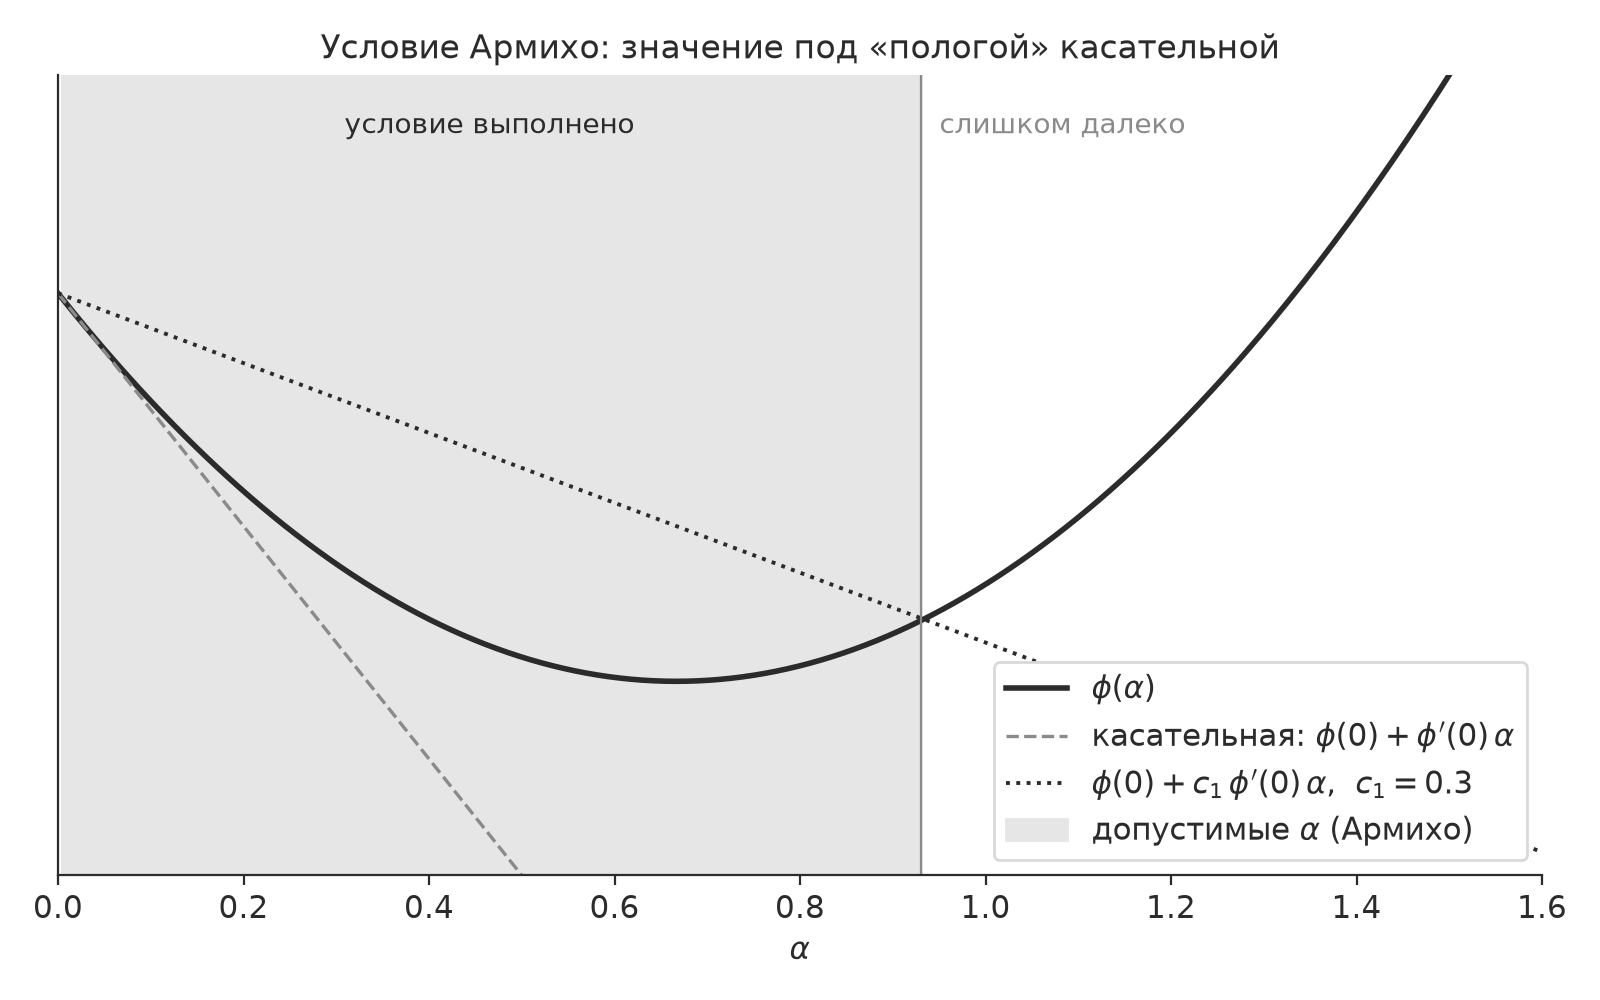
\includegraphics[width=.8\linewidth]{../../images/armijo.png}
  \end{center}

  Давайте представим, что локально функция напоминает параболу, тогда из этого ограничения следует, что если мы перейдем в точку $\alpha_k$, и она окажется на противоположной ветке параболы, то она должна находиться не слишком высоко.  То есть мы не должны уйти слишком далеко от минимума.

  Это защищает от того, чтобы мы слишком долго прыгали между левой и правой ветками и не могли сойтись.
\end{remark}
  % Условие Армихо

\InputIfFileExists{text/2084FD2F-E2AA-4081-B9D1-14CEA27EA243-before}{}{}
% generated by roam.py handbook export -- не редактировать, править заметки
% 20261007180400-условие_вульфа.org (body 86956683c9b5)

\begin{definition}[{Условие Вульфа}]\label[definition]{note:2084FD2F-E2AA-4081-B9D1-14CEA27EA243}
  Пусть $\phi: \R \rightarrow \R$, $\phi \in C^1(\R)$~--- непрерывно \hyperref[note:957FA09D-8883-40A5-B4C7-237D9F815A42]{дифференцируема}, рассмотрим отрезок $[a;b]$, такой что $\phi^{\prime}(a) < 0$ \\
  Зафиксируем $0 < c_2 < 1$.

  Условие Вульфа:
  \[| \phi^{\prime}(\alpha_k) | < c_2|\phi^{\prime}(a)|
  \]
\end{definition}

\begin{remark}[Интерпретация]
  Это условие говорит нам, что в следующей точке касательная должна быть более пологая, чем в этой. Причем умножение на $c_2$ усиливает это условие. То есть новая точка должна оказаться там, где наклон заметно меньше,~--- ближе к минимуму.

  \begin{center}
    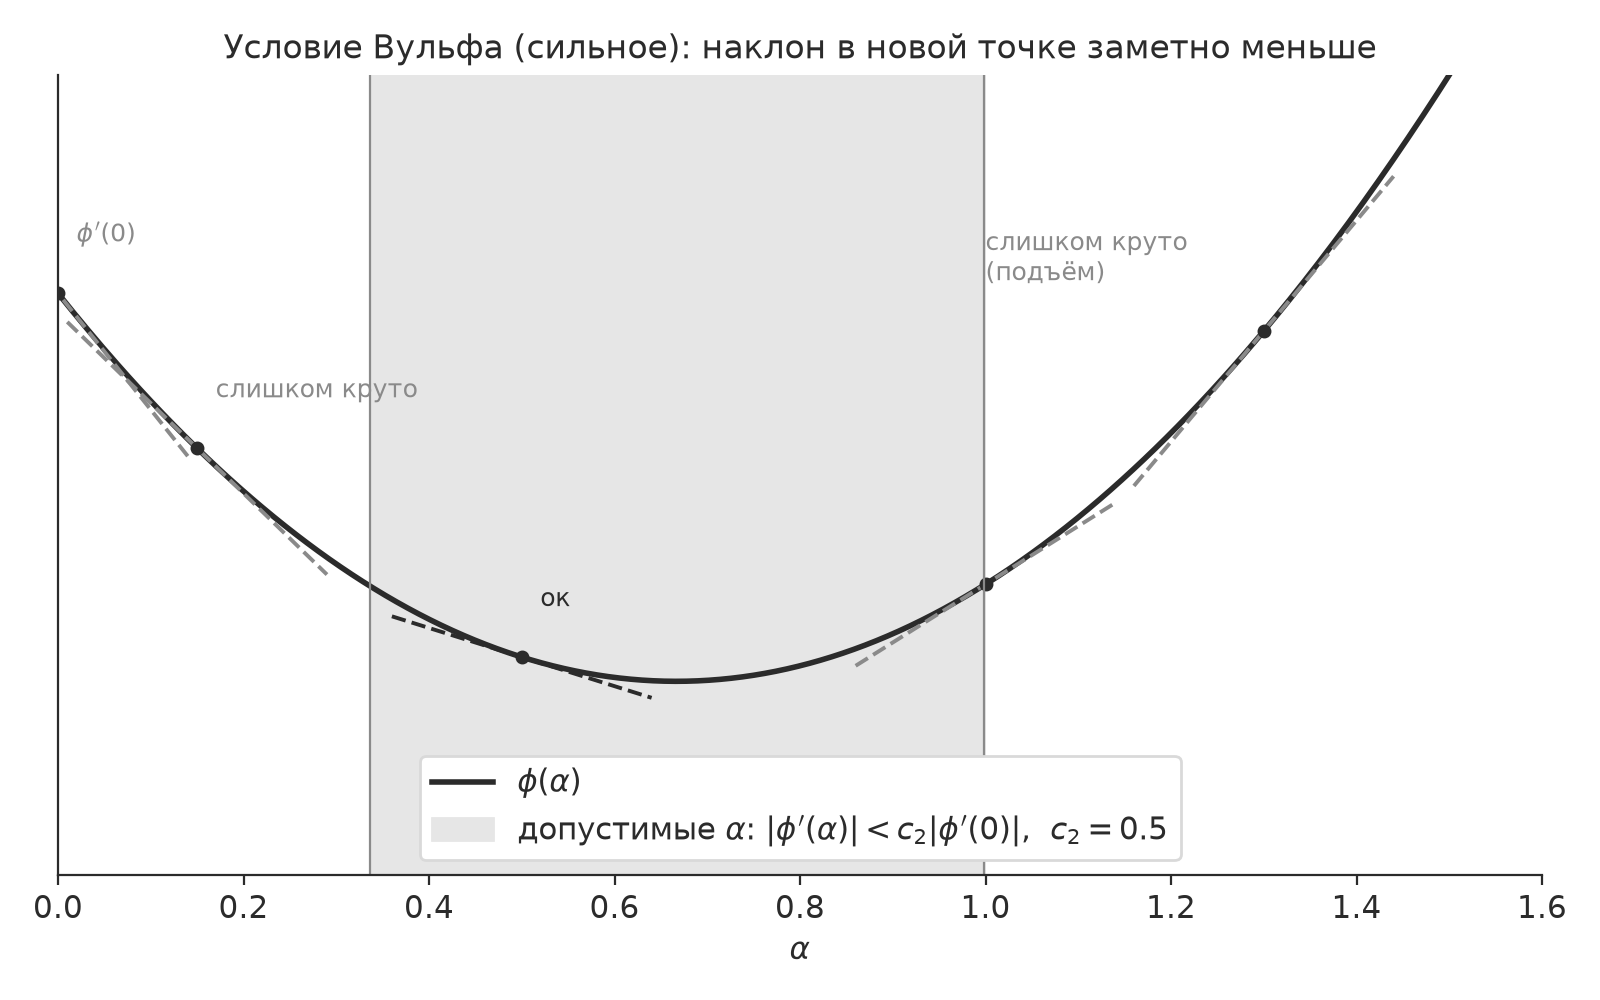
\includegraphics[width=.8\linewidth]{../../images/wolfe.png}
  \end{center}

  Получается, что это условие говорит нам: если мы выбрали $\alpha_k$ на той же ветке, то мы хотя бы должны спуститься по этой ветке достаточно глубоко. То есть мы должны прыгнуть достаточно далеко.
\end{remark}
  % Условие Вульфа -- опр. 3.3, по условию с интерпретацией

\InputIfFileExists{text/C143295F-C422-4FEE-95AD-3D6B620BC0E8-before}{}{}
% generated by roam.py handbook export -- не редактировать, править заметки
% 20261007180721-существование_шага_для_армихо_вульфа.org (body 576c97fcdd3a)

\begin{theorem}[{Существование шага для Армихо-Вульфа}]\label[theorem]{note:C143295F-C422-4FEE-95AD-3D6B620BC0E8}
  Пусть $\phi: \R \rightarrow \R$, $\phi \in C^1(\R)$ (непрерывно \hyperref[note:957FA09D-8883-40A5-B4C7-237D9F815A42]{дифференцируема}) и $\phi$ ограничена снизу;
  Требуем выполнения \hyperref[note:5330B23D-95DD-4D5D-B4A3-63EBADB1DB7D]{Условий Армихо-Вульфа} (НУО, считаем что $a = 0$).
  То есть $\phi^{\prime}(0) < 0$, $0 < c_1 < 1$, $0 < c_2 < 1$; дополнительно требуем $c_1 < c_2$.

  Тогда: $\exists \alpha^{\prime} > 0$ такое, что

  \begin{enumerate}
    \item $\phi(\alpha^{\prime}) < \phi(0) + c_1\phi^{\prime}(0)\alpha^{\prime}$
    \item $|\phi^{\prime}(\alpha^{\prime})| < c_2 |\phi^{\prime}(0)|$
  \end{enumerate}
\end{theorem}

\begin{proof}
  \proofpart{Выполнение пункта 1}
  Пусть $g(\alpha):= \phi(0) + c_1 \phi^{\prime}(0)\alpha$  -- прямая из 1 условия \\
  Заведем $\psi(\alpha) = \phi(\alpha) - g(\alpha) = \phi(\alpha) - \phi(0) - c_1 \phi^{\prime}(0)\alpha$ (функция оценки неравенства) \\
  Разложим $\phi$ по \hyperref[note:F7C9E077-9CAB-4149-83B4-67923B49E2F6]{формуле Тейлора с остаточным членом Пеано} в точке 0. $\phi(\alpha) = \phi(0) + \phi^{\prime}(0) \alpha + o(\alpha)$ \\
  Итого
  \[
  \psi(\alpha) = \phi(0) + \phi^{\prime}(0)\alpha + o(\alpha) - \phi(0) - c_1\phi^{\prime}(0)\alpha = (1 - c_1)\phi^{\prime}(0)\alpha + o(\alpha)
  \]
  Рассмотрим
  \[
  \lim_{\alpha \rightarrow 0} \frac{\psi(\alpha)}{\alpha} = \lim_{\alpha\rightarrow0} ((1-c_1)\phi^{\prime}(0) + o(1)) = (1-c_1)\phi^{\prime}(0) < 0
  \]
  Причем, несложно заметить, что $\psi(0) = 0$. Тогда предел $\lim_{\alpha \rightarrow 0} \frac{\psi(\alpha)}{\alpha} = \frac{\psi(\alpha) - \psi(0)}{\alpha} = \psi^{\prime}(0)$.

  Значит, для некоторого $\delta > 0$ при всех $\alpha \in (0;\delta)$ выполнено $\frac{\psi(\alpha)}{\alpha} < 0$, то есть $\psi < 0$ на $(0;\delta)$. Возьмем любое $\alpha^{\prime} \in (0; \delta)$: $\psi(\alpha^{\prime}) < 0$.

  Получили выполнение неравенства в $\alpha^{\prime}$

  \proofpart{Выполнение пункта 2}
  Заметим, что $\phi$~--- ограничена снизу, а $g$ убывает монотонно; Следовательно, найдется $\beta > \alpha^{\prime}$, при котором $g(\beta) < \phi(\beta)$, то есть $\psi(\beta) = \phi(\beta) - g(\beta) > 0$.

  Мы получили, что $\psi(\alpha^{\prime}) < 0$ и $\exists \beta:\  \psi(\beta) > 0$. Так как $\psi$~--- непрерывна, как разность двух непрерывных, то по \hyperref[note:6ADBECA2-157A-4C66-B4C4-F5F2AF0899AE]{теореме о промежуточном значении} у $\psi$ есть хотя бы один положительный ноль.
  Они положительные так как $\alpha^{\prime} > 0$, а $\beta > \alpha^{\prime}$.

  Пусть $\alpha^{\prime\prime}$~--- наименьший положительный ноль $\psi$ (он существует: множество нулей замкнуто, а на $(0;\delta)$ нулей нет). Тогда имеем $\psi(0) = \psi(\alpha^{\prime\prime}) = 0$. Причем $\psi$~--- дифференцируема (очев). Тогда по \hyperref[note:85DC4D66-3AE3-4619-BBEC-9A8113EBF85F]{теореме Ролля}: $\exists c \in (0; \alpha^{\prime\prime}):\ \psi^{\prime}(c) = 0$

  Рассмотрим $\psi^{\prime}(c)$:
  \[
  \psi^{\prime}(c) = \phi^{\prime}(c) - c_1\phi^{\prime}(0) = 0
  \]
  Тогда
  \[| \phi^{\prime}(c) | = c_1 | \phi^{\prime}(0) | < c_2 | \phi^{\prime}(0) |
  \]
  $c_1 < c_2$ по условию

  \proofpart{Подходит ли $c$ для 1 пункта?}
  Мы знаем, что $c \in (0; \alpha^{\prime\prime})$, а $\alpha^{\prime\prime}$~--- наименьший положительный ноль $\psi$, поэтому на $(0;\alpha^{\prime\prime})$ функция $\psi$ не обращается в ноль и по непрерывности сохраняет знак. Вблизи нуля $\psi < 0$ (пункт 1), значит $\psi < 0$ на всем $(0;\alpha^{\prime\prime})$ и $\psi(c) < 0$. Итого искомый шаг~--- $\alpha^{\prime} := c$.
\end{proof}
  % Существование шага для Армихо-Вульфа -- теорема 3.1

\InputIfFileExists{text/03E395A1-0606-49C1-978A-7275296FE023-before}{}{}
% generated by roam.py handbook export -- не редактировать, править заметки
% 20261007201907-алгоритмы_для_подбора_шага_с_условиями_армихо_вульфа.org (body 7d5635598c4e)

\begin{method}[{Алгоритмы для подбора шага с условиями Армихо-Вульфа}]\label[method]{note:03E395A1-0606-49C1-978A-7275296FE023}
  Пользуются 2 алгоритмами:

  \begin{itemize}
    \item \hyperref[note:F16921E1-67C5-4EDE-A55F-AD11D8257A69]{Backtracking} (тут шаг только уменьшают, пока он не станет соответствовать \hyperref[note:15611E05-13FC-4FB0-AE00-A4BB857A29E6]{условию Армихо})
    \item Expand \& zoom (подбирает шаг, который соответствует \hyperref[note:5330B23D-95DD-4D5D-B4A3-63EBADB1DB7D]{всем 2 условиям})
  \end{itemize}
\end{method}
  % Алгоритмы для подбора шага с условиями Армихо-Вульфа -- нет в конспекте

\InputIfFileExists{text/F16921E1-67C5-4EDE-A55F-AD11D8257A69-before}{}{}
% generated by roam.py handbook export -- не редактировать, править заметки
% 20261007202246-алгоритм_backtracking_для_подбора_шага_армихо_вульфа.org (body 4acd14827128)

\begin{method}[{Алгоритм Backtracking для подбора шага Армихо-Вульфа}]\label[method]{note:F16921E1-67C5-4EDE-A55F-AD11D8257A69}
  Алгоритм ищет шаг, который удовлетворяет \hyperref[note:15611E05-13FC-4FB0-AE00-A4BB857A29E6]{условию Армихо}.
\end{method}

\paragraph*{Алгоритм}
\begin{Verbatim}[fontsize=\small]
# Условные обозначения:
#   phi(a) = f(x + a*d) - функция по направлению d
#   dphi(a) = grad_f(x+a*d) @ d - производная по направлению d

def backtrack(phi, dphi0, alpha0=1.0, c1=1e-4, beta=0.5):
    """Шаг с условием Армихо. dphi0 = phi'(0) < 0, 0 < beta < 1"""
    phi0 = phi(0.0)
    alpha = alpha0
    while phi(alpha) > phi0 + c1 * alpha * dphi0: # Условие армихо нарушено
        alpha *= beta
    return alpha
\end{Verbatim}

\paragraph*{Почему алгоритм остановится?}
В 1 шаге доказательства теоремы \hyperref[note:C143295F-C422-4FEE-95AD-3D6B620BC0E8]{Существование шага для Армихо-Вульфа} мы доказали, что условие Армихо выполнено во всех точках интервала $(0;\delta)$. А так как $\beta^k\alpha_0 \rightarrow 0$, то при достаточно большом $k$, оно окажется в нужном интервале.

\paragraph*{Почему шаг достаточно большой?}
По \hyperref[note:FFEA1F1D-B70C-4B4A-9386-8344A2A3BBC4]{оценке убывания за шаг} для $y = x - \alpha \nabla f(x)$, где $\alpha$~--- шаг, который мы получили:
\[
f(x - \alpha \nabla f(x)) \le f(x) - \alpha \left( 1 - \frac{L\alpha}{2} \right) \|\nabla f(x)\|^2
\]

Зададим $\phi(\alpha) = f(x - \alpha \nabla f(x))$. Тогда \hyperref[note:15611E05-13FC-4FB0-AE00-A4BB857A29E6]{условие Армихо} для $\alpha_0 = 0$, $\alpha_k = \alpha$:
\[
\phi(\alpha) < \phi(\alpha_0) + c_{1}(\alpha - \alpha_0) \cdot \phi^{\prime}(\alpha_0)
\]
Подставим значения $f$
\[
f(x - \alpha \nabla f(x)) <  f(x - 0 \cdot \nabla f(x)) - c_1 \alpha \| \nabla f(x) \|^2
\]
Пользуемся тем, что
\begin{multline*}
\phi^{\prime}(\alpha) =  f^{\prime}(x - \alpha\nabla f(x))(- \alpha \nabla f(x))^{\prime}_{\alpha} = \\  - f^{\prime}(x - \alpha\nabla f(x)) \nabla f(x) = - (\nabla f(x - \alpha \nabla f(x)))^T \nabla f(x)
\end{multline*}

Тогда $\phi^{\prime}(\alpha_0) = \phi^{\prime}(0) = - (\nabla f(x))^T \nabla f(x) = - \|\nabla f(x)\|^2$

Следовательно (при $\nabla f(x) \ne 0$) условие будет выполняться при $1 - \frac{L\alpha}{2} > c_{1} \Leftrightarrow \alpha < 2 \frac{1-c_1}{L}$ \\
Заметим, что предыдущий $\alpha$ мы отвергли, следовательно шаг в $\frac{1}{\beta}$ раз больший $\alpha$ не подходит;

Итого
\[\alpha \ge \min \left\{ \alpha_0; \frac{2\beta(1-c_1)}{L} \right\}\]

То есть $\alpha$ это шаг порядка $\frac{1}{L}$.
  % Алгоритм Backtracking для подбора шага Армихо-Вульфа

\section{Многомерная оптимизация: градиентный спуск}\label{lecture:3:4}  % конспект 3.3
\InputIfFileExists{text/03-4-intro}{}{}

\InputIfFileExists{text/FFEA1F1D-B70C-4B4A-9386-8344A2A3BBC4-before}{}{}
% generated by roam.py handbook export -- не редактировать, править заметки
% 20261010131647-оценка_убывания_за_шаг_градиентного_спуска.org (body 7d72493f0803)

\begin{lemma}[{Оценка убывания за шаг градиентного спуска}]\label[lemma]{note:FFEA1F1D-B70C-4B4A-9386-8344A2A3BBC4}
  Пусть $f: \R^n \to \R$, $f \in C^{1,1}_L$ (\hyperref[note:7DD1C7AB-1A49-4675-9F21-5A16C717F670]{функция с липшицевым градиентом}), $x \in \R^n$, $\alpha > 0$ и $y = x - \alpha \nabla f(x)$~--- шаг \hyperref[note:BEEE81AD-13FC-4846-A160-C72E31760BEE]{градиентного спуска}. Тогда
  \[
  f(y) \le f(x) - \alpha \left( 1 - \frac{L\alpha}{2} \right) \|\nabla f(x)\|^2
  \]
\end{lemma}

\begin{remark}
  Убывание гарантировано при $0 < \alpha < 2/L$. Множитель $\alpha(1 - L\alpha/2)$ максимален при $\alpha = 1/L$, и тогда $f(y) \le f(x) - \frac{1}{2L}\|\nabla f(x)\|^2$~--- отсюда выбор постоянного шага $1/L$.
\end{remark}

\begin{proof}
  Воспользуемся \hyperref[note:379E4CAD-A44B-4631-8DAF-F3DC708EAEDE]{усиленным неравенством для функций с липшицевым градиентом}
  \[
  f(y) \le f(x) + \left\langle \nabla f(x); y-x \right\rangle + \frac{L}{2} \|y-x\|^2
  \]
  и подставим $y - x = -\alpha \nabla f(x)$:
  \begin{multline*}
  f(y) \le f(x) + \left\langle \nabla f(x); -\alpha \nabla f(x) \right\rangle + \frac{L}{2} \|\alpha \nabla f(x)\|^2 \\
  = f(x) - \alpha \|\nabla f(x)\|^2 + \frac{\alpha^2 L}{2} \|\nabla f(x)\|^2 = f(x) - \alpha \left( 1 - \frac{L\alpha}{2} \right) \|\nabla f(x)\|^2
  \end{multline*}
\end{proof}
  % Оценка убывания за шаг градиентного спуска -- внутри доказательства теоремы 3.2; выбор шага $1/L$

\InputIfFileExists{text/C3B64D64-D35B-42AC-B683-6736227CBBBC-before}{}{}
% generated by roam.py handbook export -- не редактировать, править заметки
% 20261003154311-сходимость_градиентного_спуска_для_функции_с_липшицевым_градиентом.org (body b801e01ac5ae)

\begin{theorem}[{Сходимость градиентного спуска для функций с липшицевым градиентом}]\label[theorem]{note:C3B64D64-D35B-42AC-B683-6736227CBBBC}
  Пусть $f: \R^n \to \R$, $f \in C_L^{1,1}$~--- \hyperref[note:7DD1C7AB-1A49-4675-9F21-5A16C717F670]{Функции с липшицевым градиентом}, и $f^{*} = \inf_x f(x) > - \infty$.
  Возьмем $\alpha_k = \frac{1}{L}$, а $x_{k+1} = x_k - \alpha_k \nabla f (x_k)$ (см. \hyperref[note:BEEE81AD-13FC-4846-A160-C72E31760BEE]{Градиентный спуск})

  Тогда: Градиентный спуск сходится~--- означает, что $\| \nabla f(x_k)\| \rightarrow 0$, причем
  \[
  \min_{0 \le i \le k} \| \nabla f(x_i)  \| \le \sqrt{\frac{2L (f(x_0) - f^{*})}{k+1}}
  \]
\end{theorem}

\begin{proof}
  По \hyperref[note:FFEA1F1D-B70C-4B4A-9386-8344A2A3BBC4]{оценке убывания за шаг} при $x = x_k$, $y = x_{k+1} = x_k - \alpha \nabla f(x_k)$:
  \[
  f(x_{k+1}) \le f(x_k) - \alpha \left( 1 - \frac{L\alpha}{2} \right) \|\nabla f(x_k)\|^2
  \]
  Подставим $\alpha = \frac{1}{L}$ (Тогда оно максимизирует $\alpha \left(1- \frac{L \alpha}{2}\right)$) \\
  Тогда
  \[
  f(x_{k+1}) \le f(x_k) - \frac{1}{L} \left( 1 - \frac{1}{2}  \right) \|\nabla f(x_k)\|^2 = f(x_k) - \frac{1}{2L} \| \nabla f(x_k)\|^2
  \]
  Давайте перенесем норму налево, а $f(x_{k+1})$ направо
  \[
  \frac{1}{2L} \|\nabla f(x_k)\|^2 \le f(x_k) - f(x_{k+1})
  \]

  Заметим, что $f(x_k) - f(x_{k+1})$ образуют телескопическую сумму:
  \[
  \sum\limits_{k=0}^n [f(x_k) - f(x_{k+1})] = f(x_0) - f(x_{n+1})
  \]
  Также заметим, что $f(x_{n+1}) \ge f^{*}$, он не меньше минимума (естественно); Тогда у нас есть такая оценка
  \[
  \sum\limits_{k=0}^n [f(x_k) - f(x_{k+1})] = f(x_0) - f(x_{n+1}) \le f(x_0) - f^{*}
  \]

  А еще мы можем это оценить снизу: через сумму норм. Тогда
  \[
  \frac{1}{2L} \sum\limits_{k=0}^n \|\nabla f(x_k)\|^2 \le \sum\limits_{k=0}^n [f(x_k) - f(x_{k+1})] \le f(x_0) - f^{*}
  \]

  Ряд $\sum\limits_{k=0}^{\infty} \|\nabla f(x_k)\|^2$ сходится (частичные суммы ограничены числом $2L(f(x_0) - f^{*})$), значит его члены стремятся к нулю: $\|\nabla f(x_k)\| \to 0$. Это первая часть утверждения. Для оценки скорости
  давайте оценим сумму норм градиентов снизу, как $n+1$ минимальных градиентов
  \[
  \frac{n+1}{2L} \min_{0 \le k \le n} \| \nabla f(x_k)\|^2 \le f(x_0) -f^{*}
  \]
  Давайте оставим только минимум слева
  \[
  \min_{0 \le k \le n} \|\nabla f(x_k)\| \le \sqrt{\frac{2L (f(x_0) - f^{*})}{n+1}}
  \]

  Правая часть стремится к нулю как $\frac{c}{\sqrt{n}}$~--- оценка \hyperref[note:A74C35E2-DDF7-4115-99B7-2448CF7C6878]{сублинейного} порядка (быстрее ли сходимость на самом деле, теорема не говорит).

  \begin{remark}
    Оценка $c/\sqrt{n}$ получена для минимума нормы по первым итерациям, а не для $\|\nabla f(x_n)\|$: сама норма градиента стремится к нулю, но не обязана убывать монотонно.
  \end{remark}
\end{proof}
  % Сходимость градиентного спуска для функций с липшицевым градиентом -- теорема 3.2

\InputIfFileExists{text/85D9D77D-13A2-42E0-BF93-AD085E0134B9-before}{}{}
% generated by roam.py handbook export -- не редактировать, править заметки
% 20261009215047-сходимость_градиентного_спуска_для_сильно_выпуклых_функции_с_липшицевым_градиентом.org (body 298e0549d12f)

\begin{theorem}[{Сходимость градиентного спуска для сильно выпуклых функций с липшицевым градиентом}]\label[theorem]{note:85D9D77D-13A2-42E0-BF93-AD085E0134B9}
  Пусть $f: \R^n \to \R$, $f \in C^{1,1}_L$ (\hyperref[note:7DD1C7AB-1A49-4675-9F21-5A16C717F670]{Функции с липшицевым градиентом}), $\mu$-\hyperref[note:22E546FC-186F-4A67-85AA-2C85DCEF9021]{сильно выпуклая}, $x^{*}$~--- её точка минимума (она \hyperref[note:51CC880D-BF19-43E2-9599-FB31A9A7367F]{существует и единственна}).
  \hyperref[note:BEEE81AD-13FC-4846-A160-C72E31760BEE]{Градиентный спуск} с шагом $\alpha_k = \frac{1}{L}$: $x_{k+1} = x_k - \frac{1}{L} \nabla f(x_k)$.

  Тогда $x_k \rightarrow x^{*}$, причем
  \[
  \| x_k -x^{*}\|^2 \le \left( 1 - \frac{\mu}{L} \right)^k \|x_0 -x^{*}\|^2
  \]
\end{theorem}

\begin{proof}
  По \hyperref[note:FFEA1F1D-B70C-4B4A-9386-8344A2A3BBC4]{оценке убывания за шаг} при $\alpha = \frac{1}{L}$ для любого $y$ имеем $f\left(y - \frac{1}{L}\nabla f(y)\right) \le f(y) - \frac{1}{2L}\|\nabla f(y)\|^2$, а слева стоит значение $f$, не меньшее минимума $f(x^{*})$. Значит
  \[
  \frac{1}{2L}\| \nabla f(y)\|^2 \le f(y) - f(x^{*})
  \]
  (то же следует из \hyperref[note:655064DF-D686-4726-83DC-6F3D67CC5B9C]{оценки для выпуклых функций с липшицевым градиентом} при $x := x^{*}$~--- так в конспекте.)

  Из \hyperref[note:1B5A3E25-56E8-4D5E-9CF6-E2731DA77604]{дифференциального критерия сильной выпуклости} следует, что
  \[
  f(y) \ge f(x) + \left\langle \nabla f(x); y-x \right\rangle + \frac{\mu}{2} \|y-x\|^2
  \]

  Пусть $x_{k+1} = x_k -\alpha \nabla f(x_k)$, где $\alpha = \frac{1}{L}$ (пока не подставляем).

  Тогда
  \[
  \| x_{k+1} - x^{*}\|^2 = \|x_k - x^{*} - \alpha \nabla f(x_k)\|^2
  = \|x_k - x^{*}\|^2 - 2 \left\langle x_k - x^{*}; \alpha \nabla f(x_k) \right\rangle + \| \alpha \nabla f(x_k)\|^2
  \]

  Заметим, что
  \[
  f(y) \ge f(x) + \left\langle \nabla f(x); y-x \right\rangle + \frac{\mu}{2} \|y-x\|^2 \Leftrightarrow -
  \left\langle \nabla f(x); y-x \right\rangle \ge f(x) - f(y) + \frac{\mu}{2} \|y-x\|^2
  \]
  Применим это для $y:=x^{*}, x:=x_{k}$.
  \[
  -\left\langle \nabla f(x_k); x^{*}-x_k \right\rangle \ge f(x_k) - f(x^*) + \frac{\mu}{2} \|x_k-x^*\|^2
  \]
  Тогда давайте занесем минус в скалярное произведение
  \[
  \left\langle \nabla f(x_k); x_k - x^{*} \right\rangle \ge f(x_k) - f(x^*) + \frac{\mu}{2} \|x_k-x^*\|^2
  \]
  Домножим все неравенство на $-1$
  \[
  - \left\langle \nabla f(x_k); x_k - x^{*} \right\rangle \le  f(x^*) - f(x_k) - \frac{\mu}{2} \|x_k-x^*\|^2
  \]

  Также заметим, что
  \[
  \| \alpha \nabla f(x_k)\|^2 = \frac{1}{L^2} \| \nabla f(x_k)\|^2
  \]
  По неравенству из спуска
  \[
  \frac{1}{L^2} \| \nabla f(x_k)\|^2   = \frac{2}{L} \cdot \frac{1}{2L} \| \nabla f(x_k)\|^2
  \le \frac{2}{L} (f(x_k) - f(x^{*}))
  \]

  Далее давайте применим эти оценки к $\|x_{k+1} - x^{*}\|^2$
  \begin{multline*}
  \| x_{k+1} - x^{*}\|^2 = \|x_k - x^{*} - \alpha \nabla f(x_k)\|^2
  = \|x_k - x^{*}\|^2 - 2 \left\langle x_k - x^{*}; \alpha \nabla f(x_k) \right\rangle + \| \alpha \nabla f(x_k)\|^2 \\
  \le \|x_k - x^{*}\|^2 + 2\alpha \left( f(x^{*}) - f(x_k) - \frac{\mu}{2} \|x_k - x^{*}\|^2\right)
  + \frac{2}{L} (f(x_k) - f(x^{*}))
  \end{multline*}

  Заменим $\alpha = \frac{1}{L}$ и сгруппируем слагаемые.
  \begin{multline*}
  \|x_k - x^{*}\|^2 + \frac{2}{L} \left( f(x^{*}) - f(x_k) - \frac{\mu}{2} \|x_k - x^{*}\|^2\right) + \frac{2}{L} (f(x_k) - f(x^{*})) = \\
  \| x_k - x^{*}\|^2 \left( 1 - \frac{\mu}{L} \right) + \frac{2}{L} (f(x^{*}) - f(x_k) + f(x_k) - f(x^{*})) = \| x_k - x^{*}\|^2 \left( 1 - \frac{\mu}{L} \right)
  \end{multline*}

  Итого получили, что
  \[
  \| x_{k+1} - x^{*}\|^2 \le \|x_k - x^{*}\|^2 \left( 1- \frac{\mu}{L} \right) \le \ ... \le
  \|x_0 - x^{*}\|^2 \left( 1- \frac{\mu}{L} \right)^{k+1}
  \]

  Так как $\mu \le L$ (\hyperref[note:3C6CF60E-0773-488E-A0B9-4D7510D456C0]{связь сильной выпуклости и липшицевости градиента}), $0 \le 1 - \frac{\mu}{L} < 1$, и правая часть стремится к нулю: $x_k \to x^{*}$.

  Получили \hyperref[note:DF2405BF-8B31-47EB-8DEF-B1A88034717C]{линейную сходимость} для \hyperref[note:C42D2C19-B35F-4C0E-AFEB-D880CBB72176]{невязки} $\|x_{k} - x^{*}\|^2$: $C = \|x_0- x^{*}\|^2$, $q = 1 -\frac{\mu}{L}$ (для самой $\|x_k - x^{*}\|$ знаменатель $q = \sqrt{1 - \mu/L}$).

  \begin{remark}
    Без сильной выпуклости (\hyperref[note:C3B64D64-D35B-42AC-B683-6736227CBBBC]{теорема для $C^{1,1}_L$}) есть лишь сублинейная оценка $c/\sqrt{k}$ для нормы градиента; сильная выпуклость даёт линейную сходимость самих точек со знаменателем $1 - \mu/L = 1 - 1/\kappa$, где $\kappa = L/\mu$~--- число обусловленности.
  \end{remark}
\end{proof}
  % Сходимость градиентного спуска для сильно выпуклых функций с липшицевым градиентом -- теорема 3.3

\noteagain{3C6CF60E-0773-488E-A0B9-4D7510D456C0}{Связь сильной выпуклости и липшицевости градиента}  % -- замечание 3.6 (было на лекции 2)

\InputIfFileExists{text/03-outro}{}{}
